\documentclass{article}
%% Change fonts to something friendly to acrobat
%%
%\usepackage{courier}
%\usepackage{times,mathptmx}
%\DeclareMathAlphabet{\bm}{OT1}{ptm}{b}{it}
\usepackage{graphicx}
\usepackage{amsmath} % used for extended formula formatting tools
\usepackage{amssymb}
\usepackage{theorem}
\usepackage{euscript}

\topmargin  0.0in
\headheight  0.15in
\headsep  0.15in
\footskip  0.2in
\textheight 8.45in

\oddsidemargin 0.56in
\evensidemargin \oddsidemargin
\textwidth 5.8in

\pagestyle{myheadings}
\markright{\bf {\em FlowPsi} User Guide (Version 1.0)}

\begin{document}


\title{{\em FlowPsi}: An ideal gas flow solver -- The User Guide.}

\author{ Edward A. Luke, Xiaoling Tong, and Rex Chamberlain}

\maketitle
\section{Introduction}

{\em FlowPsi } is an open source CFD solver that is developed
utilizing the Loci framework\cite{Luke.2005,Zhang.2009} which provides
for automatic parallelization and logical consistency checks
simplifying the design of highly parallel numerical solvers for
partial differential equations.

\section{Units}

All input into the solver is assumed to be in the international MKS
system.  For example, length is measured in meters, mass in kilograms,
time in seconds, pressure in Pascals, temperature in Kelvin, heat in
Joules, and so on.  Unless otherwise noted this standard is maintained
in all {\em FlowPsi} input and output files.  Note that {\em FlowPsi}
provides unit conversions on most inputs such that a user can input
the units that are most comfortable.  Output files are always in MKS
units, however.

\section{Problem Input}

The input to {\em FlowPsi} consists of a problem description file containing
variable definitions and postfixed with {\tt .vars}. The file
describes the boundary conditions, initial conditions, and directives
to the numerical solver. The grid file is stored in a Loci specific
``volume grid'' format that has a {\tt .vog} postfix.  A variety of
mesh conversion utilities are provided as part of the Loci framework
to convert the grid to the format used by {\em FlowPsi}.  

\subsection{Problem Description File}
\label{prob_description_file}

The problem description file (with the postfix {\tt .vars}) is used to
describe the grid, boundary conditions, initial conditions, and
numerical solution parameters.  The occurrence of the characters {\tt // }
anywhere in the file indicates a comment to the end of that line.  The
file consists of a set of variable definitions enclosed in braces.
Each variable is listed at the beginning of a line followed by a colon
and then its definition.  An example of an input file
named {\tt input.vars} is as follows:
\begin{verbatim}
{
boundary_conditions: <
                 body=viscousWall(adiabatic),
                 base=viscousWall(adiabatic),
                 BC_7=fixedMass(mdot = 0.0027 kg/s, T0=300 K) //air injection
                 BC_5=symmetry,
                 BC_6=symmetry,
                 BC_10=reflecting,
                 outflow=extrapolate,
                 inflow=supersonicInflow(p=21571.6 Pa, T=149.6 K, M=2.2)>

// initial conditions
initialConditions: < p=21571.6, T=149.6, M=0.0>
p0: 21571.6  //gage pressure reference

gridCoordinates: axisymmetric // add axisymmetric frame of reference
flowRegime: laminar
timeStepMode: steady 

plot_freq: 100
plot_modulo: 100
restart_freq:100
restart_modulo: 100
stop_iter:  5000

limiter: venkatakrishnan
Kl: 1.0

urelax: 0.20
dtmax:  1.0e-3
}
\end{verbatim} 

You can find out about all of the available input variables to {\em FlowPsi}
by using the ``{\tt -inputs}'' option to the {\em FlowPsi} executable.
These variables are also defined as follows:


\begin{enumerate}
 
\item {\tt boundary\_conditions}

This variable list is used to associate boundary surface tags in 
the grid file with a boundary condition specification.  For example:
\begin{verbatim}
boundary_conditions:  <
     Body=viscousWall(adiabatic),
     SymmetryPlane=symmetry,
     OutflowPlane=outflow(p=5005.1342psi),
     InflowPlane=supersonicInflow(p=1atm, T=500K, M=1.2) >
\end{verbatim}
Note: The last entry of this specification does not have a comma!
Also, make sure that in the grid generator program (Gridgen, for
example) you use different flags for each of the boundary surfaces
that you will want to process separately ({\it e.g.}, integrate
quantities, visualize, etc.).  Note, the terms {\tt Body}, {\tt
  SymmetryPlane}, etc.  are symbolic names given to these boundary
surfaces by the grid generator.  If the symbolic names are not
available when the grid file is converted to the {\tt vog} format,
then these names will be related to the original integer tag given to
the surface.  For example, if a surface had an integer tag of {\tt 5},
then the name {\tt BC\_5} would be given to the surface if no symbolic
name was provided.

\item {\tt initialConditions} 

  These variables define the uniform initial conditions throughout the
  domain (Note: the initial conditions are automatically read from a
  file when restarting the solver, and it is also possible to specify
  an interpolated initial conditions file - see below).  The initial
  conditions are specified by a set of flags and options as described
  in Table \ref{tab:fs}.  The variable {\tt initialConditions} is used
  to define the uniform initial values.  To describe initial
  conditions with different values in different regions, see the next
  item.  For specification of the initial conditions, only two
  thermodynamic inputs are required from the choice of {\tt P}, {\tt
    T}, or {\tt rho} and that either {\tt u} or {\tt M} is also needed
  to define velocity.  If a turbulence model is loaded, then
  additional variables may be specified in the initial conditions to
  override default values (see the turbulence model section for the
  more initial condtion information).

\begin{table}[htbp]

  \begin{centering}
    \leavevmode
  \begin{tabular}{|l|l|l|l|}
    \hline
    Variable & description & units & notes \\
    \hline\hline
    {\tt rho}      & density     & $kg/m^3$ & specified with either {\tt
    p} or {\tt T} \\
    {\tt p}        & pressure    & $Pa$     & specified with either {\tt
    T}  or {\tt rho} \\
    {\tt T}        & temperature & $K$      & specified with either {\tt
    p}  or {\tt rho} \\
    {\tt u}        & velocity    & $m/s$    & exclusive with {\tt M} \\
    {\tt M}        & Mach number &  --    & exclusive with {\tt u} \\
    \hline
  \end{tabular}
\caption{variables describing a fluid state input}
  \label{tab:fs}
  \end{centering}
\end{table}

An example for specifying the initial conditions in the {\tt .vars} file is as follows:

\begin{verbatim}
initialConditions:  <p=10 atm, T=550 R, M=0.1>
\end{verbatim}

\item {\tt initialConditionRegions}

This option is used to specify initial conditions with regions of
constant properties.  Regions can be defined using geometric
primitives such as boxes, spheres, cylinders, and so on. In the {\tt
  initialConditionRegions } specification, there are two required
options: the definition of the default initial condition state, and
the definition of a list of regions (defined by geometric
primitives).  Each geometric region can refer to other defined
states.  For example, to set up a spherical blast problem, one can
define the initial conditions using {\tt initialConditionRegions} as
follows:

\begin{verbatim}
initialConditionRegions: < 
default = state(p=1atm,T=298K,u=0),
high_pressure = state(p=1000atm,T=5000K,u=0),
regions = [ inSphere(radius=1m,center=[0,0,0],composition=high_pressure) ]
>
\end{verbatim}

The state function contains a specification of the state of the fluid
system and can contain any of the initial conditions parameters.
The regions variable describes a list of
geometric regions.  Each geometric region has a corresponding
composition which is in turn described by an assignment of a state
function.  The last specified region has priority over all previous regions.
Thus one could make a cone with a rounded outer boundary by combining
a conic region and a sphere as follows:

\begin{verbatim}
initialConditionRegions: < default = state(p=1atm,T=298K,u=0),
high_pressure1 = state(p=1000atm,T=5000K,u=0),
high_pressure2 = state(p=500atm,T=1000K,u=0),
regions = [ inSphere(radius=1m,center=[1,0,0],composition=high_pressure2),
inConic(r1=0,r2=1,p1=[-5,0,0],p2=[1,0,0],composition=high_pressure1) ]
>
\end{verbatim}

The geometric primitives currently supported are as follows:

\begin{itemize}
\item {\tt inBox}

{\tt inBox} takes two arguments, {\tt p1} and {\tt p2}, which are two
diagonally opposing corners that define the box.  The geometry is
defined as any point that lies inside of this rectangular axis aligned region.

\item {\tt inSphere}

{\tt inSphere} takes two arguments, {\tt radius} and {\tt center},
which define the sphere size and location, respectively.

\item {\tt inCylinder}

{\tt inCylinder} takes three arguments, {\tt radius}, {\tt p1}, and
{\tt p2}.  The endpoints of the axis are defined by the points {\tt
  p1} and {\tt p2}.

\item {\tt inCone}

{\tt inCone } takes four arguments.  Like {\tt inCylinder}, it uses
two endpoints of the axis, while {\tt r1} and {\tt r2} define the
respective radii at each endpoint.

\item {\tt leftPlane}

{\tt leftPlane} takes two arguments, {\tt point} and {\tt normal}.
{\tt point} defines a point on the plane, while {\tt normal} gives a
vector normal to the plane.  All points on the opposing side of the
plane (away from the normal) are included in this geometry.

\end{itemize}

\item {\tt inviscidFlux}

  Select flux formulation for the inviscid flux in the solver.  The
  selection can be ``hllc'', ``kec'', or ``ssf''.  The ``hllc'' is the
  default upwind scheme.  The ``kec'' is a second order low
  dissipation flux, and ``ssf'' is based on a fourth order skew
  symmetric scheme.  Select the ``ssf'' for LES style simulations.


\item {\tt flowRegime }

This sets the type of flow model we will be using.  This will be set
to either {\tt inviscid}, {\tt laminar}, or {\tt turbulent}.  If the
setting is {\tt turbulent} then a turbulence model will need to be
loaded using a {\tt loadModule} directive at the top of the vars file.  

\item {\tt timeStepMode }

This variable selects the time integration mode.  It is set to either
{\tt steady} or {\tt unsteady}.  In {\tt steady} mode, {\tt flowPsi }
will utilize a backward Euler time integration method with local
timestepping enabled.  For time-accurate simulations select {\tt
  unsteady} to disable local timestepping and switch to a second order
temporal integration.

\item {\tt print\_freq}

  This variable describes the frequency at which CFL numbers and integrated
  boundary condition data will be displayed on standard output.  For
  example, if this variable is set to {\tt 100}, then output will be
  generated for every time step evenly divisible by 100.
  
\item {\tt restart\_freq} 

  This variable describes the frequency at which restart files are output.
  Restart files are output in the {\tt restart/\#} directory, where
  {\tt \#} is the current iteration number (modulo {\tt
    restart\_modulo}, see next item).  This directory contains many
  files that define the entire restart state.  If you want to prevent a
  restart state from being overwritten in subsequent runs, copy this
  entire directory to a safe location.  

\item {\tt restart\_modulo} 

This variable controls the naming of the output file.  The iteration
number modulo this value will be used when outputting restart files
(overwriting files if necessary).  This can save on disk space by
limiting the maximum number of files that may exist at any given time.
It is recommended to set it to at least twice the restart frequency to
guarantee that the restart file won't become corrupted if the program
terminates while writing a restart file.


\item {\tt plot\_freq}

Outputs values that are used for generating visualizations and plots.
The {\tt extract} utility can be used to convert these files into
formats compatible with other post-processing visualization programs
such as {\em FieldView}, {\em EnSight}, or {\em Tecplot}. (See the Plot Format Converter in Section
\ref{sec:converter}).

\item {\tt plot\_modulo}

Similar to restart modulo, except applies to plot files.

\item {\tt boundary\_plot\_freq}

  The frequency that boundary information will be plotted.  Note,
  boundary plot files will be written at both {\tt plot\_freq}
  iterations and {\tt boundary\_plot\_freq} iterations.

\item {\tt plot\_output}

  Provides a comma delimited list of additional variables to output
  along with the default variables.  
%%A list of the additional variables
%%  is given in table \ref{tab:nodalextract}.

\item {\tt plot\_output\_exclusive}

  Provides a comma delimited list of additional variables to output.
  If this variable is present, then the default output variables
  will not be written unless they are included in this list.  A list
  of additional variables is given in table
  \ref{tab:extract}. %%table \ref{tab:nodalextract}.  
  Note that if you
  want to output ``put'' files for restarting put {\tt put} in this
  list and if you want to output species mixtures put {\tt mixture} in
  this list.

\item {\tt stop\_iter}

  This variable defines the iteration at which the simulation is terminated.

\item {\tt maximumRunTime}

  This variable defines the maximum running time for the
  simulation.  When this time is exceeded the code will automatically
  save restart files and terminate.  The default units
  is seconds, but the user can specify any time units.  For
  example, if one wanted to make sure the job stopped before 24 hours
  expired, you would put this in the {\tt .vars} file:
\begin{verbatim}
maximumRunTime: 23.5 hour
\end{verbatim}

\item {\tt newton\_iter}
  
  This variable defines the number of Newton iterations performed
  for each time-step.  Typically {\tt 1} for steady-state calculations,
  and {\tt >=3} for unsteady calculations.

\item {\tt fluidLinearSolver }

  This variable selects the fluid linear system solver to use to solve
  the fluid and turbulence models.  The default setting is {\tt sgs}
  which uses the built in symmetric Gauss-Seidel solver.  The setting
  {\tt fsgs} uses a fast, cache optimized, symmetric Gauss-Seidel
  solver.  It is faster than {\tt sgs} but uses more memory.  A robust
  and fast solver that is recommended is the line symmetric
  Gauss-Seidel solver which is selected by setting this variable to
  {\tt lsgs}.  This solver divides the matrix into lines and solves
  each line with a tri-diagonal solver.  The solver sweeps through
  lines similar ot the symmetric Gauss-Seidel.  For the line solver,
  some under-relaxation is employed to stabilize the solver.  In general,
  this solver is very robust and useful for high Reynolds number or
  low speed problems.  The most robust solver is the one provided by
  PetSC (if it is installed).  This solver is selected by setting this
  variable to {\tt petsc}.

\item {\tt gauss\_seidel\_iter}

  This variable defines the number of Gauss-Seidel iterations that
  will be performed when solving the linear system using {\tt sgs}.
  When this variable is set to zero, the linear solver reduces to a
  block Jacobi iteration.  Typical values are between 5-20.  Usually a
  value of 5-8 is useful for parallel simulations.

% \item {\tt LDS\_dissipationLimit} 

%   This variable limits the maximum value of the uwind blending factor.
%   The maximum value should not exceed 1 in which case the blending
%   will be fully upwind.  The Default setting of this option is 1.

% \item {\tt LDS\_ducrosFactor}

% This variable sets how much of the Ducro

\item {\tt LDS\_compFactor}

  When using the low dissipation fluxes 'kec' or 'ssf' it is necessary
  to switch to the upwind scheme around compressible features such as
  shocks.  This is input sets the sensitivity of the factor to switch
  to upwind when compressible flow conditions are detected.  The
  default value for this is 5.0.  This value is typically set
  somewhere between 1-100.  Set it to zero if these compressible
  features should not be encountered.

\item {\tt LDS\_useUpwind}

  This input will set the lower limit for the upwind blending.
  Setting this to a small positive value such as 0.2 can be used for a
  MILES type of LES subgrid model.  The default value is 0.0.

\item {\tt LDS\_nonSymmetricCoeff}

  For unstructured meshes some upwinding is needed to to stabilize the
  scheme.  Heuristic methods are used to increase the upwinding
  blending parameter when mesh cells depart form symmetric stencils.
  The larger this factor the more robust the scheme will be to poor
  mesh quality at the expense of increased dissipation. The default
  value is 2.

\item {\tt LDS\_nonSymmetricFactor}

  For unstructured meshes this controls the rate at the scheme adds
  upwinding at small angles.  A larger number will increase robustness
  at the expense of added dissipation.  the default value is 1.

\item {\tt LSGSMaxIter} 

  The maximum number of line Gauss-Seidel steps
  allowed per solve. The default is 10.

\item {\tt LSGSRelTol} 

  The residual relative error tolerance for the linear system solver
  to conclude iteration.  The default value is 0.1.  Note, that in the
  {\em FlowPsi} solver the linear system solved is only an approximation.
  Usually after some amount of residual convergence it is more
  productive to proceed to the next Newton iteration in order to
  achieve overall convergence of the PDE.  Overconverging the linear
  system solver can be non-productive as the linear system itself
  contains approximation errors.  Usually a factor of 10 reduction in
  the linear system residual is all that is needed for the Newton
  iteratons to proceed productively, but some problems will benefit
  from a more robust convergence of the approximate linearization.
  For difficult problems there may be some productivity to adjusting
  this parameter to a smaller value (while also increasing the {\tt
    LSGSMaxIter} variable).

\item {\tt LSGSAbsTol}

  The absolute error tolerance for the residual.  The default is 1e-10.

\item {\tt LSGSRelaxation}

  The under-relaxation parameter for the LSGS solver.  Usually the
  line Symmetric Gauss Seidel is unstable when solving for large
  timesteps.  An under-relaxation parameter of 0.3 (the default)
  provides stability and rapid convergence for most problems.  For
  problems where the LSGS solver diverges, a smaller setting to this
  value may allow convergence.  However, setting this value too small
  may prevent convergence in any reasonable number of iterations.

\item {\tt limiter }

  This variable describes the limiter that will be used to limit the
  MUSCL extrapolation scheme.  The current choices are {\tt
    venkatakrishnan} (default), {\tt barth}, {\tt none}, and {\tt zero}.  
  The Venkatakrishnan limiter also has a thresholding parameter
  that assists in improving accuracy and convergence.  The {\tt none}
  option disables the limiter, and this can only be used on
  sub-critical flows that do not contain discontinuities.  The
  {\tt zero} option disables higher order extrapolation (first order solution).
  Generally, the Barth limiter provides robustness while the Venkatakrishnan
  limiter provides improved accuracy and convergence characteristics.
  
\item {\tt Kl}
  
  This is the thresholding parameter for the Venkatakrishnan limiter.
  It is a problem dependent parameter that can range from $0$ to
  $100$.  When {\tt Kl} is zero, the limiter is no longer
  thresholded.  If {\tt Kl} is set to a large value, limiting is
  effectively turned off everywhere.  At an ideal setting, this
  parameter allows the limiter to be disabled in smooth regions
  permitting higher accuracy while still being applied in regions of
  discontinuities.  By default, {\tt Kl} is set to $1$.  The default
  setting should be sufficient for most uses.

\item {\tt dtmax}
  
  This variable is the global time step parameter.  

\item {\tt cflmax} 
  
  When this variable is set to a non-zero value, it enables local
  time-stepping.  Once local time-stepping is enabled, each cell's
  time-step is determined by the smallest of the following
  candidate time-steps:  1) {\tt dtmax}, 2) the time-step determined
  from {\tt cflmax}, and 3) a time-step determined from the {\tt urelax}
  (see item \ref{item:urelax}) parameter.

\item {\tt urelax} \label{item:urelax}

  This parameter limits local time-steps (when {\tt cflmax > 0})
  to a time-step that would produce no more than a {\tt urelax} factor
  change in density, pressure, and temperature.  When set to a small
  value, it should prevent occurrence of negative pressure calculations.
  The default value is 1.

\item {\tt gridCoordinates}

  The default {\tt gridCoordinates} are {\tt cartesian}, but the {\tt
    axisymmetric} option is available for 2D translated grids that are
  to be run in the axisymmetric mode.  This option replaces the pie
  slice or rotated grid approach for axisymmetric solutions.  To use
  the {\tt axisymmetric} option, the grid must be translated by an
  arbitrary distance in the $z$ direction, and the solution must be
  computed in the $x-y$ plane.  The mesh cell areas and volumes are
  adjusted to match the effect of rotating the 2D grid 360$^o$ about
  the $x$ axis, and the translation distance is ignored.  The boundary
  areas reported in the output are for the fully rotated 3D grid when
  running with {\tt gridCoordinates: axisymmetric}.  The
  correspondence between velocity components in cartesian and
  cylindrical coordinates is $(u, v, w) \rightarrow (u_z, u_r,
  u_{\theta})$, where $w \rightarrow u_{\theta}$ is the swirl
  velocity.


\item {\tt coriolis }

  If this variable is set, then the Coriolis terms are added to the
  simulation to account for a rotating frame of reference.  The
  rotation is set through the options {\tt axis} that specifies the
  rotation axis, {\tt center} that specifies the center of rotation,
  and {\tt speed} that specifies the rotation rate.  For example
  to simulate a moving reference frame that is rotating at 1000 rpm
  about the $x$-axis, one would specify:
\begin{verbatim}
coriolis: <axis=[1,0,0], center=[0,0,0], speed=1000 rpm>
\end{verbatim}
\end{enumerate}

\subsection{Boundary Condition Specifications}


The boundary conditions may be assigned as:
  {\tt inflow}, {\tt supersonicInflow},
  {\tt isentropicInflow}, {\tt fixedMass}, {\tt fixedMassOutflow},
  {\tt farfield}, {\tt outflow}, {\tt supersonicOutflow},
  {\tt extrapolate}, {\tt symmetry}, {\tt impermeable},
  {\tt reflecting}, {\tt viscousWall}, {\tt wallLaw}, {\tt periodic},
  and {\tt interface}.  When a boundary condition requires a specified thermodynamic
  state, the state specification follows the same format as the {\tt initialCondions}
  (see Table \ref{tab:fs} above).\\
  
  Notes on boundary conditions:

  \begin{list}{}{}

    
  \item {\tt inflow}

    This is a non-reflecting, characteristic-based boundary condition
    that uses the given thermodynamic state ({\it{e.g.}}, {\tt
      inflow(p=1atm, T=300K, M=0.3)}) to
    compute the inflow conditions and the boundary flux.  This
    boundary condition may be used for subsonic or supersonic inflow
    conditions.
    
  \item {\tt supersonicInflow}

    This boundary condition holds the inflow values at the given
    conditions but computes a characteristic-based flux at the
    boundary.  This condition can be used for imposing subsonic or
    supersonic inflow conditions in which the boundary flux is
    computed from a Riemann solver.

  \item {\tt isentropicInflow}

    This inflow boundary condition maintains constant entropy.  The
    user provides the total pressure and total temperature for the
    associated ``plenum'' conditions, and the inflow values that
    preserve the total properties are computed.  A typical
    multi-species input is {\tt isentropicInflow(p0=1atm, T0=300K)}.
    {\bf Note: this boundary condition is only applicable to subsonic
      inflow conditions.}

  \item {\tt fixedMass}

    This inflow boundary condition specifies the mass flow or flux
    and total temperature.  The user provides the
    {\tt mdot} ($kg/s$) or {\tt massFlux} ($kg/m^2-s$) and
    a total temperature.  A typical input is {\tt
    fixedMass(mdot=0.02 kg/sec, T0=1000 K)}.  This boundary condition
    uses the specified 3D mass rate value for axisymmetric flows in which a 2D grid
    is translated in the $z$ direction (see the {\tt gridCoordinates} input option).  {\bf Note:
    this boundary condition is only applicable to subsonic inflow conditions.}

  \item {\tt fixedMassOutflow}

    This boundary condition specifies the mass flow or flux
    at an outflow boundary.  The user provides the
    {\tt mdot} ($kg/s$) or {\tt massFlux} ($kg/m^2-s$) value only.  A typical input is {\tt
    fixedMassOuflow(mdot=0.02 kg/sec)}.  This boundary condition
    uses the specified 3D mass rate value for axisymmetric flows in which a 2D grid
    is translated in the $z$ direction (see the {\tt gridCoordinates} input option).  {\bf Note:
    this boundary condition 1) limits the outflow conditions to physically allowable values if the flow
    becomes choked and 2) extrapolates to the boundary if the flow becomes supersonic.}

  \item {\tt farfield}

    The farfield boundary condition is an inflow/outflow
    characteristic based boundary condition.  It is most suitable for
    an external flow with a farfield boundary, but it can also be used
    as a non-reflecting outflow boundary in some internal flows
    ({\it{e.g.}}, {\tt farfield(p=1atm, T=300K, M=0.3)}).  It handles
    both supersonic and subsonic flow conditions.

  \item {\tt outflow}
    
    This is a characteristic based (subsonic) condition that imposes a
    constant static pressure at the outflow boundary ({\it{e.g.}},
    {\tt outflow(p=1atm)}).  Use this boundary condition when you
    intend to hold an outflow boundary at a given pressure.  If the
    outflow becomes supersonic, this boundary condition switches to a
    supersonic outflow boundary condition ({\it{i.e.}}, {\tt
      extrapolate}) in which the pressure is no longer prescribed.
    This boundary condition can also be used to establish an
    average pressure on the outflow boundary if the {\tt pMean}
    variable is specified.  For example, {\tt outflow(pMean=1atm)}
    would establish an area averaged (mean) pressure on the boundary of one
    atmosphere.

  \item {\tt supersonicOutflow}
    
    This boundary condition extrapolates all values to the boundary
    and should only be used for fully supersonic outflow.  If the flow
    becomes subsonic, it applies a pressure reduction at the boundary
    to encourage supersonic outflow.  This condition does not require
    any arguments.  {\bf Note: This boundary condition should not be
      used when the outflow may be subsonic.}


    This boundary condition extrapolates all values to the boundary.
    It may be used for supersonic outflow conditions or to establish
    zero derivatives of velocity, pressure, and temperature in
    subsonic outflow conditions.  This boundary condition switches to
    {\tt impermeable} if the boundary becomes inflow.  This condition
    does not require any arguments.

  \item {\tt symmetry}

    This boundary condition is specifically designed for 2D or
    axisymmetric simulations.  In these cases, the 2D grid is
    extruded or rotated to form a one cell thick mesh with two
    opposing symmetry planes, and this boundary condition is the most
    efficient and robust.  For 3D symmetry planes in which more than
    one cell separates the planes, {\tt reflecting} is more accurate.
    Although {\tt symmetry} can be used in these 3D cases, it is only
    first order accurate.  This condition does not require any
    arguments.

  \item {\tt impermeable}

    This boundary condition implements a second order
    characteristic-based slip wall boundary condition.  Use this
    boundary for inviscid solid walls on structured meshes.  For
    unstructured meshes, {\tt reflecting} is better behaved.  If you
    must use impermeable for unstructured meshes, use it in first
    order mode by selecting {\tt impermeable(firstOrder)}.  The first
    order mode is also a robust option for {\tt impermeable} on any
    type of symmetry plane, including those on unstructured grids and
    2D/axisymmetric grids with one cell between the planes.  This
    condition does not require any arguments ({\tt firstOrder} is
    optional).

  \item {\tt reflecting}

    This boundary condition implements a second order reflecting
    boundary condtion where the interior solution is reflected through
    the boundary normal to the exterior.  This boundary condition can
    be used to implement symmetry planes or impermeable boundary
    conditions, and it does not require any arguments.
    {\bf Note: reflecting should not be used to implement symmetry
    planes when there is only one cell between the planes as it can become
    unstable.}

  \item {\tt viscousWall}

    {\sloppy 
    This boundary condition implements the no-slip boundary condition
    for modeling viscous boundary layers.  Generally this boundary
    condition requires a viscous stretched mesh.  The {\tt viscousWall}
    boundary condition may be adiabatic {\tt viscousWall(adiabatic)},
    specified heat flux to the fluid {\tt viscousWall(qwall=-1000 watt/m/m)}
    (the minus sign denotes that the heat flux is into the domain since the
    boundary normal is positive pointing outward),
    specified temperature, {\tt viscousWall(Twall=400 K)}, prescribed (see notes
    on prescribed boundary specifications), or used to
    interface to other models, {\tt viscousWall(interface)}, for
    example in conjugate heat transfer.  For turbulent computations with a rough wall
    the sand grain roughness height ($k_s$ in meters) may also be specified,
    {\tt viscousWall(Twall=400 K, ks = 1e-5)}.
    {\bf Note: This boundary condition requires normal grid spacing of $y^+ \sim 1$ to
    achieve accurate solutions.}
}
                               
  \item {\tt periodic}

    This boundary condition is used to specify a periodic condition
    between pairs of boundaries which are identified using the same
    name.  One periodic boundary specification in the pair specifies the
    transformation between the boundaries, which may be either
    translation or rotation.  Translation is specified through a
    translation vector, and rotation is specified by a center of rotation,
    an axis of rotation, and a rotation angle.

\begin{verbatim}
    // Translated periodic boundary conditon
    BC_1=periodic(name="A", translate=[.8,0,0]),
    BC_2=periodic(name="A"),
    // rotated periodic boundary condition
    BC_3=periodic(name="B", center=0, vector=[1,0,0], 
                            rotate=30 deg),
    BC_4=periodic(name="B"),
\end{verbatim}
\end{list}

\subsubsection{ Notes on Vector Value Inputs }

Vector values (such as inflow boundary condition velocities or directed Mach
numbers) can be input in both Cartesian and spherical coordinates.  By
default, if only a single value is assigned to the vector,
it is assumed that this value points in the $x$ coordinate
direction.  A Cartesian vector is assigned by providing a list of
three values for the $x$, $y$, and $z$ components, respectively, enclosed in square
brackets, {\tt [~]}.  For example:
\begin{verbatim}
(u = [0,20 m/s, 0]) // Velocity in the +y direction
\end{verbatim}
The magnitude of the vector and the keyword {\tt normal} may also
be used to specify that the velocity is normal to the boundary:
\begin{verbatim}
(u = 20 m/s,normal) // Velocity normal to the boundary
\end{verbatim}
Likewise, we can specify the velocity using a polar notation of {\tt
polar(mag,$\Theta$,$\Psi$)} where the final vector is given by $u =
\left[ mag*cos(\Theta)*cos(\Psi),mag*sin(\Theta)*cos(\Psi),mag*sin(\Psi)\right]$.
For example:
\begin{verbatim}
(u = polar(20 meters/second,5 deg, 0)) // 5 degrees angle of attack
\end{verbatim}
The definition of the polar angles and the resulting $u$, $v$, and $w$ velocity components are shown for a right-handed Cartesian coordinate system in Fig. \ref{polar}.

\begin{figure}[htbp]
\begin{center}
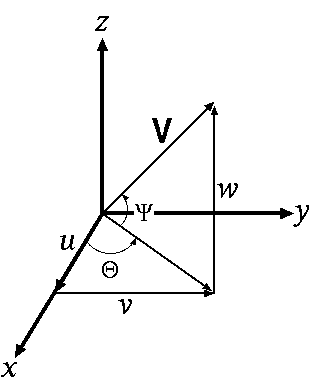
\includegraphics[width=5cm]{polar}
\caption{Definition of the polar angles used to specify the velocity components.}
\label{polar}
\end{center}
\end{figure}



\subsubsection{ Notes on Inflow Velocity Specifications}

A typical inflow boundary might be specified as:
\begin{verbatim}
  inflow(p=5000.0 psi,T=273 K,u=100, normal)
\end{verbatim}
but there are also two possible specifications for rotating flows: rigid body rotation
(helical flows) and a fixed swirling flow angle.  Rigid body rotation
is specified using the {\tt rotAxis}, {\tt rotCenter}, and {\tt
rotSpeed} boundary condition options, where {\tt rotAxis} is a vector
that defines the axis of rotation, {\tt rotCenter} is a point on the
rotation axis, and {\tt rotSpeed} is the rotational speed given by
default in revolutions per minute (rpm).  The rotation is defined by the
right-hand rule, thus a positive rotation speed about the $x$-axis {\tt
rotAxis} will produce positive $z$ components of velocity when the value
of $y$ is positive.

Alternatively, it is possible to specify a fixed swirl angle whereby
the direction of the velocity will rotate about a center axis.  This
is done using the specification of {\tt swirlAxis}, {\tt
swirlCenter}, and {\tt swirlAngle}.  The specification is similar to
the rotating flow specification, with the specified rotating flow
conforming to a right-handed coordinate system.

Both rigid body rotation and swirling flows can be specified for any
inflow boundary condition ({\tt inflow}, {\tt supersonicInflow}, {\tt farfield}, {\tt fixedMass},
and {\tt isentropicInflow}).  When these conditions are specified, the
direction of the velocity vector is modified to conform to the
rotating conditions, but the magnitude of the velocity is preserved.
For {\tt fixedMass} and {\tt isentropicInflow}, best results
will be achieved if the boundary surface is planar and normal to the
axis of rotation.  The following are some examples:

\begin{verbatim}
  inflow(p=5000.0 psi, T=274 K, u=100 m/s, 
         swirlAxis=[1,0,0], swirlCenter=[-1,0,0], swirlAngle=5deg),
  fixedMass(mdot=1kg/s, T0=300K, 
            rotAxis=[0,1,0], rotCenter=[0,0,0], 
            rotSpeed=3000 rotations/minute),
\end{verbatim}

\subsubsection{ Notes on Setting Viscous Boundary Velocity }

A tangential velocity can be specified on viscous wall boundaries for
simulating wall translation and rotation.  To specify the translational
velocity, use the {\tt Uwall} parameter.  A rotating viscous wall is
specified using the {\tt rotAxis}, {\tt rotCenter}, and {\tt rotSpeed}
options, similar to rotating inflows.  A moving wall velocity
can be specified for either viscousWall or wallLaw boundary
conditions.  In addition, only the tangential part of the specified
velocity is used in the viscous velocity specification.  

{\center \it Examples}

A moving lid with a constant linear velocity is specified as:
\begin{verbatim}
  wallLaw(adiabatic, Uwall=[1,0,0]), // Wall moving at 1 m/s to right
\end{verbatim}
A rotating wall can be specified as:
\begin{verbatim}
  viscousWall(Twall=300K, rotSpeed=100 rpm, 
              rotAxis=[0,0,1], rotCenter=0),
\end{verbatim}
where the rotation axis is the $z$ axis.


\subsubsection{Integrated Forces and Moments}
\label{integrated_fm}

{\em FlowPsi} provides the integrated forces and moments about a moment
reference center specified by the user (the default moment center is
the origin of the coordinate axes).  The output for specific BCs as
well as all of the viscous walls is placed in the standard output as
well as in special files located in the \verb!/output! directory.  The
output file naming convention and the file format are discussed below.

The user specifies a moment reference center in the \verb!.vars! file for each BC over which integrated forces and moments are required.  For example,
\begin{verbatim}
  BC_4 = viscousWall(adiabatic, momentCenter = [1., 0.5, 0.])
\end{verbatim}
locates the moment reference center for \verb!BC_4! at \verb!(1.,0.5,0.)! meters (the default units are meters).

Both the inviscid pressure and viscous shear stresses are integrated
over each BC.  For axisymmetric flows in which a 2D grid is translated
in the $z$ direction\footnote{see the {\tt gridCoordinates} input
  option for further information on computing axisymmetric flows with
  2D translated grids.}, the integration is over the 3D surface area
resulting from a 360$^o$ rotation about the $x$-axis, and the
integrations over the boundary area are computed accordingly.  For the
BCs on which a \verb!momentCenter! is specified, {\em FlowPsi} also
computes the moments for each of these force contributions.  The
forces and moments are resolved into the three coordinate directions
($x,y,z$).  Note that for the inviscid pressure contribution, the
force actually integrated is ({\it{$p - p_{ref}$}}), where $p_{ref}$
is the user input gauge pressure ({\tt .vars} file input {\tt p0})
(default $p_{ref}$ = 0).

The integrated fluxes for a specific boundary are placed in a file named \verb!/output/flux_BC4.dat!, for example.  The output format in this file is:
\begin{verbatim}
iteration, simulation time, mass flux, Fx, Fy, Fz, energy flux, area
\end{verbatim}
where \verb!Fx, Fy, Fz! are the total momentum fluxes (viscous plus inviscid) in each coordinate direction.  Similarly, the moments are placed in a file named \verb!/output/moment_BC4.dat!, and the file format is:
\begin{verbatim}
iteration, simulation time, Mx, My, Mz, RefMx, RefMy, RefMz
\end{verbatim}
where \verb!Mx, My, Mz! are the actual moments ($N$-$m$) relative to the defined \verb!momentCenter!, and \verb!RefMx, RefMy, RefMz! are the reference moments based on the integration of ({\it{$p - p_{ref}$}}) about the \verb!momentCenter!.

The force integrations over each BC surface are defined as follows:

\begin{equation}
F_x = \int{d\textbf{F} \cdot n_x dA}
\end{equation}

\begin{equation}
F_y = \int{d\textbf{F} \cdot n_y dA}
\end{equation}

\begin{equation}
F_z = \int{d\textbf{F} \cdot n_z dA},
\end{equation}
where $d\textbf{F}$ is the sum of the viscous and inviscid momentum fluxes on a surface with area $dA$, and ($n_x,n_y,n_z$) are the components of the surface normal vector.  The moment integrations are:
\begin{equation}
\textbf{M} = - \int{ \bf{(r - r_0)} \times \textbf{F} \textit{dA}} ~ ,
\end{equation}
where $\bf{r_0}$ is the user specified \verb!momentCenter! vector, and
$\bf{r}$ is the face center location of $dA$.  The {\em flowPsi}
output contains the ($x,y,z$) components of the total moment vector
$\textbf{M}$.  For axisymmetric flows in which the 2D grid is
translated in the $z$ direction, $F_x$ and $F_y$ take on the
integrated value while $F_z = 0$.  Similarly, $M_x = M_y = 0$, and
$M_z$ takes the integrated value.  Note that the moment integration is
consistent with the aerodynamic convention for pitch, roll, and yaw
({\it{i.e.}}, positive moments occur for pitch up, roll to the right,
and yaw to the right when viewed from the pilot's perspective).

%% \subsubsection{ Notes on Boundary Surface Integrations}

%% The code outputs integrated momentum, mass, and energy fluxes across
%% each boundary.  In addition an integrated moment of any given boundary
%% condition can be provided by specifying the momentCenter in the
%% specific boundary condition.  For example:

%% \begin{verbatim}
%%     BC_1=viscousWall(adiabatic,momentCenter=[0,0,0])
%% \end{verbatim}


\section{{\em FlowPsi} Pre- and Post-processing Utilities}

\subsection{{\em FlowPsi} Pre-processing Utilities}

\subsubsection{\tt ugrid2vog}

This converter allows one to convert {\it SolidMesh} or {\tt aflr3}
mesh files to the volume grid representation used by {\em FlowPsi}.  This
command can be run in parallel using mpirun for faster processing of
large meshes.  By default, the command will detect if the input file is
binary or ASCII, but you can force it to read a binary {\tt .b8.ugrid}
file using the {\tt -b} option.  The converter also has a {\tt -o}
option to disable optimizations that would change the numbering of
nodes and cells in the mesh from the given {\tt ugrid} file.
Generally this option would only be used if it is important for the
grid conversion to preserve the original node ordering.  Additionally,
you may input the units of the ugrid mesh (default is meters) with the option {\tt -in}
for inches, {\tt -ft} for feet, {\tt -cm} for centimeters, or {\tt -mm} for milimeters.  If another
unit is needed, you may use the {\tt -Lref} option. For example, if the
input grid named {\tt "wingsection.b8.ugrid"} is
non-dimensionalized with respect to a reference length
of 1.57 inches, you would use the command:
\begin{verbatim}
ugrid2vog -Lref "1.57 inch" wingsection
\end{verbatim}

\subsubsection{\tt xdr2vog}

This converter allows one to convert the older XDR format mesh files
to the volume grid representation used by {\em FlowPsi}.  This command can be
run in parallel using mpirun for faster processing of large meshes.
The converter has a {\tt -o} option to disable optimizations that
would change the numbering of nodes and cells in the mesh from the
given XDR mesh file.  Additionally, you may input the units of the XDR
mesh with the option {\tt -in} for inches, {\tt -ft} for feet, {\tt
  -cm} for centimeters, or {\tt -mm} for milimeters.  With no option,
{\tt xdr2vog} will assume the input is in meters.  The {\tt -Lref}
option can be used as with {\tt ugrid2vog} to specify other unit
systems.  

\subsubsection{\tt vogmerge}

The {\tt vogmerge} utility allows one to combine VOG file grids, apply
geometric transformations to the grids, rename boundary tags, and
apply volume tags.  Use options 

\begin{verbatim}
vogmerge -g input.vog -zscale -1 -g input.vog -o combine.vog
\end{verbatim}

Note that the geometric transform options are applied to the grid of
the preceding {\tt -g} options.  If many geometric transforms are
specified, then they are applied in the given order.  Finally, for
each grid, one may apply a volume tag using the {\tt -tag} option.
This is used when creating grids for simulations using relative
motion.  For example, to perform a simulation on turbo-machinery that included a rotor and stator section, one would generate two grids, one for each component, and then merge them using the following vogmerge command:
\begin{verbatim}
vogmerge -g rotor.vog -tag rotor -g stator.vog -tag stator -o turbo.vog
\end{verbatim}
Once can then prescribe different motions to each grid using the {\tt
  componentMotion} variable in the {\tt .vars} file using the volume tags
{\tt rotor} and {\tt stator}.

Executing {\tt vogmerge} without any options will provide a usage guide.
The current options to {\tt vogmerge} are:

\begin{table}[htbp]
\begin{center}
\begin{tabular} {|l|l|}
\hline
option & description\\
\hline\hline
  {\tt -g} {\it gridfile}           & Specify input grid filename \\
  {\tt -o} {\it gridfile}           & Specify output grid filename \\
  {\tt -xshift} {\it value}         & translate grid in x-coordinate\\
  {\tt -yshift} {\it value}         & translate grid in y-coordinate\\
  {\tt -zshift} {\it value}         & translate grid in z-coordinate\\
  {\tt -xscale} {\it value}         & scale grid in x-coordinate\\
  {\tt -yscale} {\it value}         & scale grid in y-coordinate\\
  {\tt -zscale} {\it value}         & scale grid in z-coordinate\\
  {\tt -scale}  {\it value}         & scale grid in all coordinates\\
  {\tt -xrotate} {\it value}        & rotate about x-axis (degrees)\\
  {\tt -yrotate} {\it value}        & rotate about y-axis (degrees)\\
  {\tt -zrotate} {\it value}        & rotate about z-axis (degrees)\\
  {\tt -bc} {\it oldname}{\tt ,}{\it newname} & rename boundary surface\\
  {\tt -glue} {\it bcname}          & glue this boundary to a matching bc\\
  {\tt -tag} {\it name}             & specify volume tag for input grid\\
\hline
\end{tabular}
\end{center}
\end{table}

\subsubsection{\tt cobalt2vog}

The {\tt cobalt2vog} grid converter will convert an ASCII unformatted {\it Cobalt 60} grid format file and convert it into a VOG grid suitable for use with {\em FlowPsi}.  The extension on the cobalt grid should be {\tt cog}.

\subsubsection{\tt plot3d2vog}

The {\tt plot3d2vog} grid converter will convert multi-block plot3d files into an VOG file format compatible with {\em FlowPsi}. 

\subsubsection{\tt fluent2vog}

The {\tt fluent2vog} grid converter will convert fluent {\tt .msh} files to the VOG file format for use with {\em FlowPsi}.

\subsubsection{\tt ccm2vog}

The {\tt ccm2vog} grid converter will convert Star CCM+ grids to the VOG file format for use with {\em FlowPsi}.


\subsubsection{\tt vogcheck}

The {\tt vogcheck} utility is a grid quality assesment tool for {\em FlowPsi}.
This program can be run in parallel for larger grids using mpirun.
The program outputs an overall assesment of the grid quality in the
range of {\tt UNUSABLE}, {\tt marginal}, {\tt poor}, {\tt good}, and {\tt
  excellent}.  A grid that is identified as {\tt UNUSABLE} will
probably not be useful for {\em FlowPsi} simulations.  Grids marked as {\tt
  marginal} may provide numerical robustness problems for {\em FlowPsi}.  It is
suggested that the user query the cause of poor mesh quality for these
grids.  Grids identified as {\tt poor} may be acceptable for
running with {\em FlowPsi}, but accuracy will probably be degraded in some
regions.  Any grid marked as {\tt good} or {\tt excellent} has a mesh
quality that is suitable for high quality solutions using {\em FlowPsi}.

To query the mesh quality, one can extract the mesh quality measures
from {\tt vogcheck} from iteration {\tt 0}.


\subsection{{\em FlowPsi} Post-processing utilities}

\subsubsection{Probe Output}

The {\em FlowPsi} code can output variables at a specified location to a file every
iteration using probes.  There is no limit to the number of probes allowed.
The specification in the {\tt .vars} file is:
\begin{verbatim}
probe: <probe1=[0,0,0],probe2=[1,0,1]>
\end{verbatim}
where the units of the point are in meters if units are not explicitly
specified with the point locations.  Probes will generate output files
in the form {\tt probeX.dat}, where {\tt X} is the probe number.
The file contains lines with the following information:
\begin{verbatim}
  <ncycle> <stime> <T> <p> <rho> <a> [ <U> ] [ <pos> ] <dist> <mass fractions>
\end{verbatim}
where:
\begin{verbatim}
  <ncycle> is the iteration number of the simulation
  <stime> is the simulation time
  <T> is the temperature
  <p> is the pressure
  <rho> is the density
  <a> is the sound speed
  <U> is the velocity vector
  <pos> is the position of the probe
  <dist> is the distance between the probed value and the position given in the
         input file.
\end{verbatim}

\subsubsection{Plot Format Converter}
\label{sec:converter}
See the {\tt plot\_freq} item for an explanation of how to generate data
for visualization in the {\tt output} directory.  These files are annotated by the
iteration number (modulo the {\tt plot\_modulo} value).  Once generated, the
{\tt extract} program can be used to generate various plot files for post
processing programs such as {\it FieldView},{\it EnSight}, {\it
TecPlot}, and {\it 2dgv}.  The first argument to {\tt extract} specifies
which post processing software format to use.
Table \ref{tab:extractpost} gives a list of the
currently supported post processing selectors for {\tt extract}.  Other
options may follow that are specific to the particular post processor.
The user then provides the problem name (this is the name of the {\em FlowPsi}
{\tt .vars} file without the {\tt .vars} extension),
the iteration number to extract from, and
a list of variables to extract.  The default variables output by {\em FlowPsi}
are given in table \ref{tab:extract}.  The 2dgv post processing
package will only allow the specification of a single variable, while
all others support visualization of multiple scalar and vector values.
The form of an extract command is:

\begin{verbatim}
extract -<package> [options] <problem name> <time step> <variable(s)>
\end{verbatim}

Note that documentation of how to use {\tt extract} can also be obtained by
executing the command {\tt extract} without any arguments.


\begin{table}[htbp]
  \begin{center}
    \leavevmode
    \begin{tabular}{|l|l|}
      \hline
      post-processor option & purpose \\
      \hline
      {\tt -fv} & {\it FieldView} postprocessing\\
      {\tt -en} & {\it EnSight} postprocessing\\
      {\tt -tec} & {\it TecPlot} postprocessing\\
      {\tt -2d} & {\it 2dgv} postprocessing\\
      {\tt -cut} & Dump a cutting plane for {\it 2dgv} postprocessing\\
      {\tt -ascii} & Dump selected nodal data to an ASCII file\\
      {\tt -mean} & Generate mean and variance from family of variables\\
      {\tt -surf} & Extract boundary surface mesh\\
      \hline
    \end{tabular}
    
    \caption{extract post-processor selectors}
    \label{tab:extractpost}
  \end{center}
\end{table}

\begin{table}[htbp]
  \begin{center}
    \leavevmode
    \begin{tabular}{|l|l|}
      \hline
      Key & function \\
      \hline
      r & density \\
      p & $log_{10}$(pressure) \\
      P & actual pressure in SI units \\
      u & fluid speed \\
      0, 1, 2 & Cartesian components of fluid velocity \\
      v & velocity vector \\
      m & Mach number \\
      t & temperature \\
      a & sound speed \\
      tau & wall shear stress (vector) \\
      taumag & wall shear stress magnitude (scalar)\\
      qdot & wall heat flux \\
      tw & wall temperature \\
      pw & wall pressure \\
      bt & boundary temperature \\
      bpg & boundary gage pressure \\
      br & boundary density \\
      mdot & boundary mass flux \\
      \hline
    \end{tabular}
    
    \caption{{\tt extract} command keys}
    \label{tab:extract}
  \end{center}
\end{table}

The {\em FlowPsi} code will optionally output other scalar and vector data
when these variables are provided in the {\tt plot\_output} list
in the {\tt .vars} file.  
%%The scalar variables that can be optionally written
%%by {\em FlowPsi} are given in Table \ref{tab:nodalextract}, and the vector
%%variables are given in Table \ref{tab:vectorextract}.  
For example, to
extract the turbulence model scalars {\tt k}, {\tt w}, and {\tt tmu},
one would place the following in the {\tt .vars} file:
\begin{verbatim}
// Note, no spaces between variables, just commas
plot_output: k,w,tmu
\end{verbatim}

Now the variables can be extracted for visualization with {\it FieldView} for the case {\tt plume} at iteration {\tt 100} using the command:
\begin{verbatim}
extract -fv plume 100 k w tmu
\end{verbatim}


\subsection{Surface Data Output Options}

By default {\em FlowPsi} outputs data for volume nodal data and surface facet
information.  For very large meshes or time accurate simulations where
frequent output is required, the size of the volume data can become
prohibitive.  To facilitate more control over the amount of output
data {\em FlowPsi} produces, users can instead choose to write out surface data
for a specific subset of surfaces, variables, and times.  By default
individual surface data is not written out, but the output for any
boundary surface can be enabled by adding the variable {\tt plotFreq}
and {\tt plotVars}.  The variable {\tt plotFreq} tells the frequency
of plotting for that boundary surfaces whereas {\tt plotVars} is set
set to a list of variables that will be output for that boundary
surface.  For example, if one wanted to output surface pressures and
temperatures every 10 cycles for a viscous wall boundary one could
enter in the {\tt boundary\_conditions} line:
\begin{verbatim}
bladerow = viscousWall(adiabatic, plotFreq=10, plotVars=[pg,t]),
\end{verbatim}

In addition to boundary surface data, {\em FlowPsi} can also output clip
surfaces in the form of clip planes or isosurfaces.  The clip surface
capability is enabled by adding the variables {\tt clipFreq} and {\tt
  clipSurfaces} to the vars file.  The {\tt clipFreq} variable provides an
integer which will be the frequency of clip surface output, while the
{\tt clipSurfaces} gives a list of surface names with clipping
specifications.  The clipping specification can either be a {\tt
  plane} or an {\tt isosurface}.  For a clip plane the specification
requires a {\tt point} on the plane and the {\tt normal} vector of the
plane.  The iso-surfaces specifications gives a variable assignment
where the iso-surface will be computed.  An example of clip surfaces
is given in the specification:

\begin{verbatim}
clipFreq: 25
clipSurfaces: < zcut10 = plane(point=[0,0,10],normal=[0,0,1]),
                t1000  = isosurface(t=1000),
                t0500  = isosurface(t=500)>
\end{verbatim}

The previous example will generate cut surfaces every 25 timesteps
where the cut surfaces include the surface named ``zcut10'' which is
the plane formed by $z=10$, the ``t1000'' isosurface where temperature
is 1000 Kelvin and the ``t500'' isosurface where temperature is 500
Kelvin.  Note, the input for the isosurface command cannot accept unit
specification and instead will always be interpreted in terms of
{\em FlowPsi}'s output default which is the MKS unit system.  Also note, any
variable that was specified for plotting on the volume mesh (those
listed in {\tt plot\_output} or {\tt plot\_output\_exclusive} will be
written out for these surfaces.

\subsection{Mean and Variance Output}

For hybrid RANS/LES or DES simulations, it is useful to compute mean
and variances of output variables.  There are two methods provided
to allow users to extract this type of information from a
simulation: offline and online.  The offline approach is implemented
as part of the {\tt extract} utility with the {\tt -mean} option.  The
extract utility can read in a sequence of output scalars, vectors, or
mixtures that were written out by {\em FlowPsi} and compute mean and
variance values which are then written back out to the output
directory.  The {\tt extract} utility can then be used to visualize
the resulting mean and  variance values.  To
extract these values, use the argument {\tt -mean} followed by {\tt
  -end} with the ending iteration and {\tt -inc} with the iteration
increment.  Extract starts with the usual given extract iteration number and
averages consecutive plot files at the provided increment until the
ending iteration is reached.  The mean values are then written to the
output directory as the variable with {\tt Mean} appended for the mean
and {\tt Var} for the variance.  For vector valued variables, the
covariance is also output as {\tt Cuv}, {\tt Cuw}, and {\tt Cvw} for the
covariance of the {\it x-y}, {\it x-z}, and {\it y-z} components,
respectively.  These variables can then be extracted in the usual way
for visualization.

The online method for mean and variances is enabled by adding the
following line to the top of your {\tt .vars} file (before the first brace, \{ ):

\begin{verbatim}
loadModule: onlineStats
\end{verbatim}

In the {\tt .vars} file, you will also need to add a definition for
the averaging window size using the {\tt meanFreq} variable.  The
average will automatically reset when the window size is reached.
Alternatively, the code can perform exponential averaging if the
variable {\tt useExponentialMean} is set to {\tt on}.  In the
exponential averaging approach, the averaging weight is computed based
on the window provided by {\tt meanFreq}.  When online averaging is
enabled, the code will output the variables listed in table
\ref{tab:onlinestats}.  Note that these variance values are the square
of the RMS value.  Also not that the velocity mean and variances are
Favre averaged while

\begin{table}[htbp]
  \begin{center}
    
    \leavevmode
    \begin{tabular}{|l|l|}
      \hline
      Key & function \\
      \hline
      {\tt tmean} & average temperature \\
      {\tt tvar} & variance in temperature \\
      {\tt pgmean} & mean gage pressure \\
      {\tt pgvar} & variance in gage pressure\\
      {\tt rmean} & mean density\\
      {\tt umean} & Favre mean velocity vector\\
      {\tt uvar} & Favre variance in velocity components\\
      {\tt ucovar} & Favre covariance of velocity components\\
      \hline
    \end{tabular}
    
    \caption{variables output by the {\tt onlineStats} module}
    \label{tab:onlinestats}
  \end{center}
\end{table}




\bibliography{guide}
\bibliographystyle{unsrt}

\end{document}




